% MH1812 — Chapter 6: Recurrence (0->100 ground-up)
\chapter[Recurrences]{Recurrences: Induction Proofs and Closed Forms}
\label{ch:recurrence}

\begin{quote}
\emph{``To understand recursion, you must first understand recursion.''} Recurrence relations describe sequences where each term depends on earlier ones --- the mathematical shadow of every recursive program.
\end{quote}

\noindent\fbox{\parbox{\dimexpr\linewidth-2\fboxsep-2\fboxrule}{%
\textbf{From zero: sequences that define themselves.} We start with ``next = function of previous'' (Fibonacci, factorial, Hanoi), see why naive recursion explodes, then solve recurrences to closed forms and prove them by induction.}}
\vspace{0.4em}

\section*{Learning Outcomes}
After this chapter you will be able to:
\begin{enumerate}[label=(L\arabic*)]
    \item write recurrences from recursive algorithms and combinatorial descriptions;
    \item solve linear recurrences by iteration/expansion and characteristic equations;
    \item guess and verify closed forms by induction (including strong);
    \item analyse divide-and-conquer recurrences informally;
    \item connect recurrences to induction proofs and generating functions (preview).
\end{enumerate}

% ============================================================
\section{What Is a Recurrence?}
\label{sec:what-is-recurrence}
A \emph{recurrence} (or recursion) defines $a_n$ in terms of earlier $a_k$ ($k<n$) plus base cases. Example: factorial $a_0=1$, $a_n=n\cdot a_{n-1}$; Fibonacci $F_0=0,F_1=1,F_n=F_{n-1}+F_{n-2}$; Tower of Hanoi $H_0=0$, $H_n=2H_{n-1}+1$.

Recursive algorithms induce recurrences on running time: e.g.\ binary search $T(n)=T(n/2)+O(1)$.

\begin{figure}[h]\centering
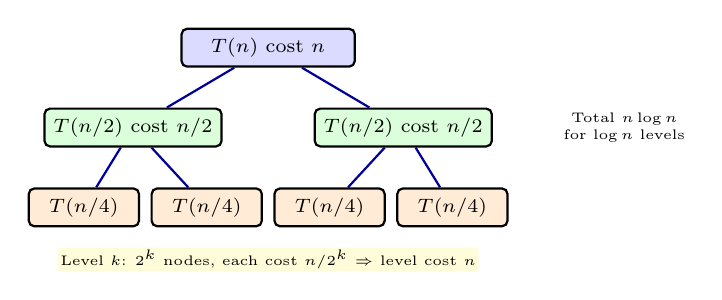
\begin{tikzpicture}[scale=0.78,every node/.style={font=\scriptsize}]
% Recursion tree for T(n)=2T(n/2)+n
\node[draw,thick,fill=blue!14,rounded corners=2pt,minimum width=2.2cm] (root) at (0,2.0) {$T(n)$ cost $n$};
\node[draw,thick,fill=green!14,rounded corners=2pt,minimum width=1.8cm] (l) at (-2.2,0.7) {$T(n/2)$ cost $n/2$};
\node[draw,thick,fill=green!14,rounded corners=2pt,minimum width=1.8cm] (r) at (2.2,0.7) {$T(n/2)$ cost $n/2$};
\node[draw,thick,fill=orange!16,rounded corners=2pt,minimum width=1.4cm] (ll) at (-3.0,-0.6) {$T(n/4)$};
\node[draw,thick,fill=orange!16,rounded corners=2pt,minimum width=1.4cm] (lr) at (-1.0,-0.6) {$T(n/4)$};
\node[draw,thick,fill=orange!16,rounded corners=2pt,minimum width=1.4cm] (rl) at (1.0,-0.6) {$T(n/4)$};
\node[draw,thick,fill=orange!16,rounded corners=2pt,minimum width=1.4cm] (rr) at (3.0,-0.6) {$T(n/4)$};
\draw[thick,blue!60!black] (root)--(l); \draw[thick,blue!60!black] (root)--(r);
\draw[thick,blue!60!black] (l)--(ll); \draw[thick,blue!60!black] (l)--(lr);
\draw[thick,blue!60!black] (r)--(rl); \draw[thick,blue!60!black] (r)--(rr);
\node[font=\tiny,fill=yellow!15,rounded corners=1pt,inner sep=1pt] at (0,-1.45) {Level $k$: $2^k$ nodes, each cost $n/2^k$ $\Rightarrow$ level cost $n$};
\node[font=\tiny,align=center] at (5.8,0.7) {Total $n\log n$\\for $\log n$ levels};
\end{tikzpicture}
\caption{Recursion tree for $T(n)=2T(n/2)+n$. Summing level costs gives $n$ per level $\times\log n$ levels.}
\label{fig:recursion-tree}
\end{figure}

Solving means finding a \emph{closed form} with no recursion, e.g.\ $H_n=2^n-1$.

\section{Solving by Iteration (Unrolling)}
\label{sec:iteration}
Unroll until pattern emerges, sum the series, prove by induction.

\begin{example}[Hanoi]
$H_n=2H_{n-1}+1$, $H_0=0$. Then $H_n=2(2H_{n-2}+1)+1=2^2H_{n-2}+2+1=\cdots=2^nH_0+\sum_{i=0}^{n-1}2^i=2^n-1$.
\end{example}

\begin{theorem}[Arithmetic recurrence]
$a_n=a_{n-1}+c$, $a_0$ given $\Rightarrow a_n=a_0+cn$.
\end{theorem}

\begin{theorem}[Geometric + constant]
$a_n=r\cdot a_{n-1}+c$, $r\neq1$ $\Rightarrow a_n=r^na_0+c\frac{r^n-1}{r-1}$ (geometric sum).
\end{theorem}

\begin{figure}[h]\centering
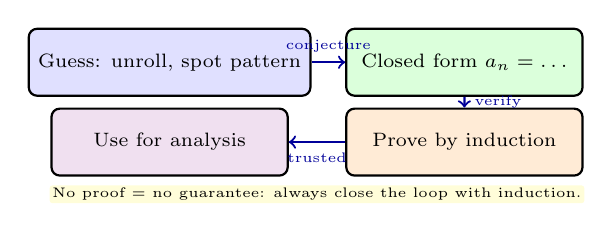
\begin{tikzpicture}[scale=0.78,every node/.style={font=\scriptsize}]
% Iteration vs induction verification
\node[draw,thick,rounded corners=3pt,fill=blue!12,minimum width=3.0cm,minimum height=0.85cm,align=center] (guess) at (0,1.6) {Guess: unroll, spot pattern};
\node[draw,thick,rounded corners=3pt,fill=green!14,minimum width=3.0cm,minimum height=0.85cm,align=center] (closed) at (4.8,1.6) {Closed form $a_n=\dots$};
\node[draw,thick,rounded corners=3pt,fill=orange!16,minimum width=3.0cm,minimum height=0.85cm,align=center] (prove) at (4.8,0.3) {Prove by induction};
\node[draw,thick,rounded corners=3pt,fill=violet!12,minimum width=3.0cm,minimum height=0.85cm,align=center] (use) at (0,0.3) {Use for analysis};
\draw[->,thick,blue!60!black] (guess)--(closed) node[midway,above,font=\tiny] {conjecture};
\draw[->,thick,blue!60!black] (closed)--(prove) node[midway,right,font=\tiny] {verify};
\draw[->,thick,blue!60!black] (prove)--(use) node[midway,below,font=\tiny] {trusted};
\node[font=\tiny,fill=yellow!15,rounded corners=1pt,inner sep=1pt] at (2.4,-0.55) {No proof $=$ no guarantee: always close the loop with induction.};
\end{tikzpicture}
\caption{Workflow: iterate to conjecture, induct to certify.}
\label{fig:iterate-induct}
\end{figure}

Induction proofs for recurrences are routine: base checks closed form at $n_0$; step substitutes IH into recurrence to get $n+1$ case.

\section{Linear Homogeneous Recurrences}
\label{sec:linear-homog}
For $a_n=c_1a_{n-1}+c_2a_{n-2}$ (order $2$, constant coefficients), try $a_n=r^n$: characteristic equation $r^2-c_1r-c_2=0$ with roots $r_1,r_2$.

\begin{theorem}[Second-order linear]
If $r_1\neq r_2$ then $a_n=\alpha r_1^n+\beta r_2^n$ for constants $\alpha,\beta$ from bases. If $r_1=r_2=r$ then $a_n=(\alpha+\beta n)r^n$.
\end{theorem}

\begin{example}[Fibonacci closed form (Binet)]
$F_n=F_{n-1}+F_{n-2}$, $r^2=r+1\Rightarrow r=(1\pm\sqrt5)/2$. So $F_n=\frac{1}{\sqrt5}\left[\left(\frac{1+\sqrt5}2\right)^n-\left(\frac{1-\sqrt5}2\right)^n\right]$. Exponential growth $\approx\phi^n/\sqrt5$.
\end{example}

\begin{example}[Non-homogeneous]
$a_n=2a_{n-1}+1$ has homogeneous part $A2^n$ plus particular constant $a=-1$: $a_n=A2^n-1$, base gives $A=1$ for $a_0=0$.
\end{example}

\begin{lstlisting}[language=Python]
# Verify closed form vs recurrence by induction check (testing)
def H_rec(n): return 0 if n==0 else 2*H_rec(n-1)+1
def H_closed(n): return 2**n - 1
print([H_rec(n)==H_closed(n) for n in range(10)])

# Fibonacci via recurrence vs Binet
import math
phi=(1+5**0.5)/2; psi=(1-5**0.5)/2
def fib_closed(n): return round((phi**n - psi**n)/5**0.5)
fib=lambda n: 0 if n==0 else 1 if n==1 else fib(n-1)+fib(n-2)
print([fib(n)==fib_closed(n) for n in range(12)])
\end{lstlisting}

\begin{figure}[h]\centering
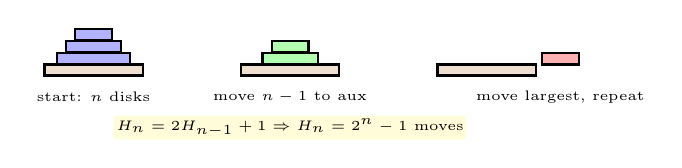
\begin{tikzpicture}[scale=0.78,every node/.style={font=\scriptsize}]
% Hanoi towers small visual
\foreach \i in {0,1,2} {\draw[thick,fill=brown!25] (\i*3.2,0) rectangle++(1.6,0.18);}
\foreach \w/\y in {1.2/0.18,0.9/0.38,0.6/0.58} {\draw[thick,fill=blue!30] (0.8-\w/2,\y) rectangle++(\w,0.18);}
\foreach \w/\y in {0.9/0.18,0.6/0.38} {\draw[thick,fill=green!30] (4.0-\w/2,\y) rectangle++(\w,0.18);}
\draw[thick,fill=red!30] (8.4-0.6/2,0.18) rectangle++(0.6,0.18);
\node[font=\tiny] at (0.8,-0.35) {start: $n$ disks};
\node[font=\tiny] at (4.0,-0.35) {move $n-1$ to aux};
\node[font=\tiny] at (8.4,-0.35) {move largest, repeat};
\node[font=\tiny,fill=yellow!15,rounded corners=1pt,inner sep=1pt] at (4.0,-0.85) {$H_n=2H_{n-1}+1\Rightarrow H_n=2^n-1$ moves};
\end{tikzpicture}
\caption{Tower of Hanoi intuition: to move $n$ disks, move $n-1$ aside, move largest, move $n-1$ back.}
\label{fig:hanoi}
\end{figure}

\begin{remark}[Master preview]
Divide-and-conquer $T(n)=aT(n/b)+f(n)$ has similar tree analysis; full Master theorem appears in SC2001. The iteration idea already predicts $n^{\log_b a}$ vs.\ $f(n)$ dominance.
\end{remark}


\begin{theorem}[Telescoping sum view]
Unrolling $a_n=r a_{n-1}+c$ yields $a_n=r^n a_0+c\sum_{i=0}^{n-1}r^i$. This is the discrete analogue of solving a linear ODE.
\end{theorem}

\begin{example}[Compound interest]
$A_n=(1+r)A_{n-1}$ with $A_0$ principal gives $A_n=A_0(1+r)^n$ --- pure geometric recurrence.
\end{example}

\begin{theorem}[First-order linear general]
$a_n=p_n a_{n-1}+q_n$ with $p_n\neq0$ solves to $a_n=\left(\prod_{i=1}^{n}p_i\right)a_0+\sum_{k=1}^{n}q_k\prod_{i=k+1}^{n}p_i$ by forward substitution.
\end{theorem}

\section{Induction Proofs for Closed Forms}
\label{sec:induction-recurrence}
Every closed form must be certified by induction because pattern-spotting is not proof. Template: let $P(n)$ be ``$a_n=$ closed$(n)$''. Base $P(n_0)$ by direct check; inductive step $P(k)\Rightarrow P(k+1)$ by substituting $P(k)$ into the recurrence and algebra.

\begin{example}[Detailed induction]
Claim: $a_n=2^n-1$ solves $a_0=0$, $a_n=2a_{n-1}+1$. Base $a_0=1-1=0$. IH $a_k=2^k-1$. Then $a_{k+1}=2a_k+1=2(2^k-1)+1=2^{k+1}-1$.
\end{example}

\begin{remark}[Strong induction for order 2]
For $F_n=F_{n-1}+F_{n-2}$, both $P(k)$ and $P(k-1)$ are needed, so use strong induction or weak with strengthened hypothesis $Q(k)=P(k)\land P(k-1)$.
\end{remark}

\begin{lstlisting}[language=Python]
# Strong induction check for Fibonacci identity sum F_i = F_{n+2}-1
def fib(n):
    a,b=0,1
    for _ in range(n): a,b=b,a+b
    return a
for n in range(10):
    assert sum(fib(i) for i in range(n+1)) == fib(n+2)-1
print("Fib identity holds for n<10")
\end{lstlisting}


\begin{example}[Second-order with repeated root detail]
$a_n=4a_{n-1}-4a_{n-2}$, $a_0=1,a_1=4$: $r^2-4r+4=(r-2)^2\Rightarrow r=2$ double. So $a_n=(\alpha+\beta n)2^n$. Bases: $1=\alpha$, $4=(\alpha+\beta)2\Rightarrow\beta=1$, hence $a_n=(1+n)2^n$.
\end{example}

\begin{theorem}[Particular solution for polynomial forcing]
If $a_n=c_1a_{n-1}+c_2a_{n-2}+p(n)$ with $p$ polynomial degree $d$, try particular $q(n)$ polynomial degree $d$ (times $n^k$ if root collision).
\end{theorem}

\begin{remark}[Why induction after guessing is mandatory]
Unrolling suggests $a_n=2^n-1$ but does not prove it --- pattern could break at $n=100$ (e.g.\ $n^2+n+41$ prime trap). Induction closes the gap.
\end{remark}

\begin{lstlisting}[language=Python]
# Solving linear recurrence via characteristic roots (numeric)
import cmath
def solve_order2(c1,c2,a0,a1,n):
    # a_n = c1*a_{n-1}+c2*a_{n-2}
    disc=c1*c1+4*c2
    r1=(c1+cmath.sqrt(disc))/2
    r2=(c1-cmath.sqrt(disc))/2
    if abs(r1-r2)<1e-9:
        r=r1
        # a_n = (alpha+beta*n)*r^n
        alpha=a0
        beta=(a1/r - alpha) if r!=0 else 0
        return (alpha+beta*n)*(r**n)
    else:
        # solve alpha+beta=a0, alpha*r1+beta*r2=a1
        beta=(a1-a0*r1)/(r2-r1)
        alpha=a0-beta
        return alpha*(r1**n)+beta*(r2**n)
print([round(solve_order2(1,1,0,1,n).real) for n in range(10)])
\end{lstlisting}

Recurrences are the discrete analogue of differential equations, describing next from now.
Unrolling reveals pattern, but only induction certifies the closed form for all $n$.
Hanoi's $2^n-1$ moves show how exponential growth emerges from a simple $2T(n-1)+1$ rule.
Arithmetic recurrences add a constant each step, geometric ones multiply, mixed ones do both.
Characteristic equations turn linear recurrences into polynomial roots, an algebraic shortcut.
Repeated roots need an extra $n$ factor, reflecting the degeneracy of the trial solution.
Particular solutions handle forcing terms like constants or polynomials, completing the general solution.
Generating functions encode the whole sequence in a power series, a uniform method for all linear recurrences.
Divide-and-conquer recurrences foreshadow the Master theorem, central to algorithm analysis.
Fibonacci's closed form via $\phi^n$ shows linear recurrences can hide irrational numbers that cancel to integers.
Recurrences are the discrete analogue of differential equations, describing next from now.
Unrolling reveals pattern, but only induction certifies the closed form for all $n$.
Hanoi's $2^n-1$ moves show how exponential growth emerges from a simple $2T(n-1)+1$ rule.

\begin{example}[Merge sort recurrence]
$T(n)=2T(n/2)+O(n)$ unrolls to $O(n\log n)$ --- the recursion tree of Ch.~6 predicts the SC2001 Master theorem case 2.
\end{example}

\begin{theorem}[Generating function preview]
Recurrence $a_n=2a_{n-1}+1$ has OGF $A(x)=\sum a_nx^n =\frac{x}{(1-2x)(1-x)}$; partial fractions recover $2^n-1$.
\end{theorem}

Arithmetic recurrences add a constant each step, geometric ones multiply, mixed ones do both.
Characteristic equations turn linear recurrences into polynomial roots, an algebraic shortcut.
Repeated roots need an extra $n$ factor, reflecting the degeneracy of the trial solution.
Particular solutions handle forcing terms like constants or polynomials, completing the general solution.
Generating functions encode the whole sequence in a power series, a uniform method for all linear recurrences.
Divide-and-conquer recurrences foreshadow the Master theorem, central to algorithm analysis.
Fibonacci's closed form via $\phi^n$ shows linear recurrences can hide irrational numbers that cancel to integers.
Recurrences are the discrete analogue of differential equations, describing next from now.
Unrolling reveals pattern, but only induction certifies the closed form for all $n$.
Hanoi's $2^n-1$ moves show how exponential growth emerges from a simple $2T(n-1)+1$ rule.
Arithmetic recurrences add a constant each step, geometric ones multiply, mixed ones do both.

\section{Worked Example: Solving a Non-Homogeneous Recurrence End-to-End}
Solve $a_0=2$, $a_n=3a_{n-1}+4$ ($n\ge1$). Iteration: $a_n=3^n\cdot2+4\sum_{i=0}^{n-1}3^i=2\cdot3^n+4\frac{3^n-1}{2}=2\cdot3^n+2(3^n-1)=4\cdot3^n-2$. Prove by induction: base $n=0$ gives $4-2=2$ ok. IH $a_k=4\cdot3^k-2$, then $a_{k+1}=3(4\cdot3^k-2)+4=4\cdot3^{k+1}-6+4=4\cdot3^{k+1}-2$. Works.

Compare to homogeneous $b_n=3b_{n-1}$ which would be $b_n=2\cdot3^n$. The constant $4$ adds a particular solution $-2$ (solve $A=3A+4\Rightarrow A=-2$). General $=$ homogeneous $+$ particular.

% ============================================================
\section{Chapter Notes}
Recurrences model recursive code, population growth, and financial compounding. Characteristic equations are linear algebra in disguise (eigenvalues). Generating functions (not covered) give a uniform solver.

% ============================================================
\section{Exercises}
\label{sec:ch06-exercises}
\begin{enumerate}[label=E6.\arabic*, leftmargin=*, itemsep=0.6em]
\item \textbf{Unrolling.} Solve $a_n=3a_{n-1}+2$, $a_0=1$ by iteration; prove your closed form by induction. Do the same for $a_n=a_{n-1}+n$, $a_0=0$.
\item \textbf{Hanoi proof.} Prove by induction that $H_n=2^n-1$ is minimal. Show any solution needs at least $2^n-1$ moves (the largest disk must move once).
\item \textbf{Characteristic equation.} Solve $a_n=5a_{n-1}-6a_{n-2}$ with $a_0=0,a_1=1$. Solve $a_n=4a_{n-1}-4a_{n-2}$ with $a_0=1,a_1=4$ (repeated root).
\item \textbf{Fibonacci identities.} Prove $F_0+\cdots+F_n=F_{n+2}-1$ and $F_n\ge2^{n/2-1}$ by induction (strong where needed).
\item \textbf{Divide-and-conquer.} Let $T(1)=1$, $T(n)=2T(n/2)+n$ for $n$ power of $2$. Unroll to guess $T(n)=n\log_2 n+n$, prove by induction.
\end{enumerate}
% End of Chapter 6
